\documentclass{article}
\usepackage[paperwidth=16.8cm,paperheight=8.8cm,margin=1mm]{geometry}
\usepackage{amsmath,amssymb}
\usepackage{xcolor}
\usepackage{tikz}
\usetikzlibrary{arrows.meta,positioning,shapes.geometric,calc}
\pagestyle{empty}

\definecolor{brickred}{RGB}{192,57,43}
\definecolor{forestgreen}{RGB}{39,174,96}
\definecolor{navyblue}{RGB}{41,128,185}
\definecolor{charcoal}{RGB}{44,62,80}
\definecolor{cloudgray}{RGB}{236,240,241}
\definecolor{amber}{RGB}{243,156,18}

\begin{document}
\noindent
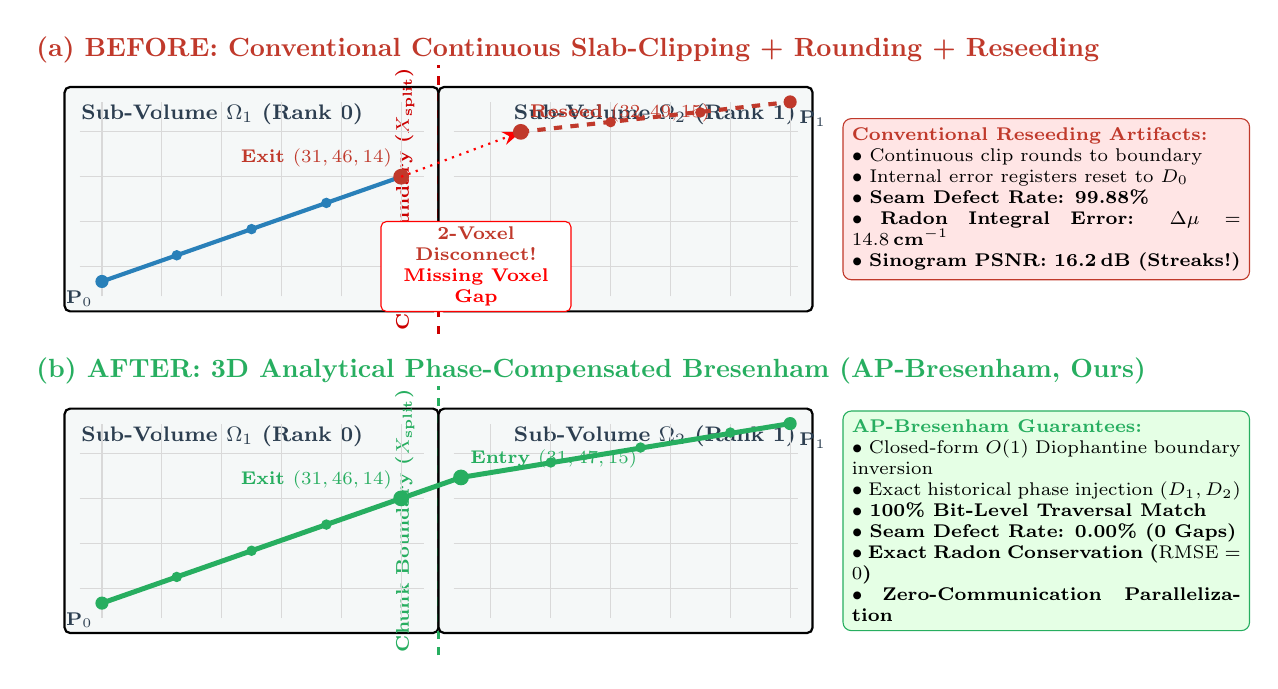
\begin{tikzpicture}[>=Stealth, font=\sffamily\small, scale=0.95, every node/.style={transform shape}]

% ==============================================================================
% TOP PANEL (a): BEFORE (Conventional Decoupled Pipeline)
% ==============================================================================
\node[anchor=west, font=\bfseries\normalsize, text=brickred] at (0, 7.3) 
    {(a) BEFORE: Conventional Continuous Slab-Clipping + Rounding + Reseeding};

% Chunk 1 Box
\draw[thick, fill=cloudgray!50, rounded corners=2pt] (0.5, 3.8) rectangle (5.5, 6.8);
\node[anchor=north west, font=\footnotesize\bfseries, text=charcoal] at (0.6, 6.7) {Sub-Volume $\Omega_1$ (Rank 0)};

% Boundary Line
\draw[very thick, dashed, red!80!black] (5.5, 3.5) -- (5.5, 7.1);
\node[anchor=south, font=\scriptsize\bfseries, text=red!80!black, rotate=90] at (5.3, 5.3) {Chunk Boundary ($X_{\text{split}}$)};

% Chunk 2 Box
\draw[thick, fill=cloudgray!50, rounded corners=2pt] (5.5, 3.8) rectangle (10.5, 6.8);
\node[anchor=north east, font=\footnotesize\bfseries, text=charcoal] at (10.4, 6.7) {Sub-Volume $\Omega_2$ (Rank 1)};

% Voxel grid lines inside Chunk 1
\foreach \x in {1.0, 1.8, 2.6, 3.4, 4.2, 5.0} {
    \draw[gray!30, line width=0.4pt] (\x, 4.0) -- (\x, 6.6);
}
\foreach \y in {4.4, 5.0, 5.6, 6.2} {
    \draw[gray!30, line width=0.4pt] (0.7, \y) -- (5.3, \y);
}

% Voxel grid lines inside Chunk 2
\foreach \x in {6.2, 7.0, 7.8, 8.6, 9.4, 10.2} {
    \draw[gray!30, line width=0.4pt] (\x, 4.0) -- (\x, 6.6);
}
\foreach \y in {4.4, 5.0, 5.6, 6.2} {
    \draw[gray!30, line width=0.4pt] (5.7, \y) -- (10.3, \y);
}

% Ray in Chunk 1
\draw[line width=1.5pt, navyblue] (1.0, 4.2) -- (5.0, 5.6);
\fill[navyblue] (1.0, 4.2) circle (2.5pt) node[below left, font=\scriptsize, text=charcoal] {$\mathbf{P}_0$};
\fill[navyblue] (2.0, 4.55) circle (2pt);
\fill[navyblue] (3.0, 4.9) circle (2pt);
\fill[navyblue] (4.0, 5.25) circle (2pt);
\fill[brickred] (5.0, 5.6) circle (3pt) node[above left, font=\scriptsize\bfseries, text=brickred] {Exit $(31, 46, 14)$};

% The Seam Dislocation / Gap
\draw[thick, red, dotted, ->] (5.0, 5.6) -- (6.6, 6.2);
\node[draw, red, fill=white, inner sep=2pt, rounded corners=2pt, font=\scriptsize\bfseries] at (6.0, 4.4) 
    {\parbox{2.4cm}{\centering \textcolor{brickred}{2-Voxel Disconnect!}\\ \scriptsize Missing Voxel Gap}};

% Ray in Chunk 2 (Dislocated and slope changed)
\fill[brickred] (6.6, 6.2) circle (3pt) node[above right, font=\scriptsize\bfseries, text=brickred] {Reseed $(32, 49, 15)$};
\draw[line width=1.5pt, brickred, dashed] (6.6, 6.2) -- (10.2, 6.6);
\fill[brickred] (7.8, 6.33) circle (2pt);
\fill[brickred] (9.0, 6.46) circle (2pt);
\fill[brickred] (10.2, 6.6) circle (2.5pt) node[below right, font=\scriptsize, text=charcoal] {$\mathbf{P}_1$};

% Callout: Reset accumulator error
\node[draw=brickred, fill=red!10, rounded corners=3pt, font=\scriptsize, anchor=west] at (10.9, 5.3) {
    \parbox{5.2cm}{
        \textbf{\textcolor{brickred}{Conventional Reseeding Artifacts:}}\\
        $\bullet$ Continuous clip rounds to boundary\\
        $\bullet$ Internal error registers reset to $D_0$\\
        $\bullet$ \textbf{Seam Defect Rate: 99.88\%}\\
        $\bullet$ \textbf{Radon Integral Error: $\Delta \mu = 14.8$\,cm$^{-1}$}\\
        $\bullet$ \textbf{Sinogram PSNR: 16.2\,dB (Streaks!)}
    }
};

% ==============================================================================
% BOTTOM PANEL (b): AFTER (3D AP-Bresenham Ours)
% ==============================================================================
\node[anchor=west, font=\bfseries\normalsize, text=forestgreen] at (0, 3.0) 
    {(b) AFTER: 3D Analytical Phase-Compensated Bresenham (AP-Bresenham, Ours)};

% Chunk 1 Box
\draw[thick, fill=cloudgray!50, rounded corners=2pt] (0.5, -0.5) rectangle (5.5, 2.5);
\node[anchor=north west, font=\footnotesize\bfseries, text=charcoal] at (0.6, 2.4) {Sub-Volume $\Omega_1$ (Rank 0)};

% Boundary Line
\draw[very thick, dashed, forestgreen] (5.5, -0.8) -- (5.5, 2.8);
\node[anchor=south, font=\scriptsize\bfseries, text=forestgreen, rotate=90] at (5.3, 1.0) {Chunk Boundary ($X_{\text{split}}$)};

% Chunk 2 Box
\draw[thick, fill=cloudgray!50, rounded corners=2pt] (5.5, -0.5) rectangle (10.5, 2.5);
\node[anchor=north east, font=\footnotesize\bfseries, text=charcoal] at (10.4, 2.4) {Sub-Volume $\Omega_2$ (Rank 1)};

% Voxel grid lines inside Chunk 1
\foreach \x in {1.0, 1.8, 2.6, 3.4, 4.2, 5.0} {
    \draw[gray!30, line width=0.4pt] (\x, -0.3) -- (\x, 2.3);
}
\foreach \y in {0.1, 0.7, 1.3, 1.9} {
    \draw[gray!30, line width=0.4pt] (0.7, \y) -- (5.3, \y);
}

% Voxel grid lines inside Chunk 2
\foreach \x in {6.2, 7.0, 7.8, 8.6, 9.4, 10.2} {
    \draw[gray!30, line width=0.4pt] (\x, -0.3) -- (\x, 2.3);
}
\foreach \y in {0.1, 0.7, 1.3, 1.9} {
    \draw[gray!30, line width=0.4pt] (5.7, \y) -- (10.3, \y);
}

% Ray in Chunk 1
\draw[line width=1.8pt, forestgreen] (1.0, -0.1) -- (5.0, 1.3);
\fill[forestgreen] (1.0, -0.1) circle (2.5pt) node[below left, font=\scriptsize, text=charcoal] {$\mathbf{P}_0$};
\fill[forestgreen] (2.0, 0.25) circle (2pt);
\fill[forestgreen] (3.0, 0.6) circle (2pt);
\fill[forestgreen] (4.0, 0.95) circle (2pt);
\fill[forestgreen] (5.0, 1.3) circle (3pt) node[above left, font=\scriptsize\bfseries, text=forestgreen] {Exit $(31, 46, 14)$};

% Seamless 26-connected transition across boundary
\draw[line width=1.8pt, forestgreen] (5.0, 1.3) -- (5.8, 1.58);
\fill[forestgreen] (5.8, 1.58) circle (3pt) node[above right, font=\scriptsize\bfseries, text=forestgreen] {Entry $(31, 47, 15)$};

% Ray in Chunk 2
\draw[line width=1.8pt, forestgreen] (5.8, 1.58) -- (10.2, 2.3);
\fill[forestgreen] (7.0, 1.78) circle (2pt);
\fill[forestgreen] (8.2, 1.98) circle (2pt);
\fill[forestgreen] (9.4, 2.18) circle (2pt);
\fill[forestgreen] (10.2, 2.3) circle (2.5pt) node[below right, font=\scriptsize, text=charcoal] {$\mathbf{P}_1$};

% Callout: Exact AP-Bresenham phase injection
\node[draw=forestgreen, fill=green!10, rounded corners=3pt, font=\scriptsize, anchor=west] at (10.9, 1.0) {
    \parbox{5.2cm}{
        \textbf{\textcolor{forestgreen}{AP-Bresenham Guarantees:}}\\
        $\bullet$ Closed-form $O(1)$ Diophantine boundary inversion\\
        $\bullet$ Exact historical phase injection $(D_1, D_2)$\\
        $\bullet$ \textbf{100\% Bit-Level Traversal Match}\\
        $\bullet$ \textbf{Seam Defect Rate: 0.00\% (0 Gaps)}\\
        $\bullet$ \textbf{Exact Radon Conservation ($\mathrm{RMSE} = 0$)}\\
        $\bullet$ \textbf{Zero-Communication Parallelization}
    }
};

\end{tikzpicture}
\end{document}
